\documentclass[oneside]{scrbook}
\KOMAoptions{fontsize=11pt, paper=a4}     
\KOMAoptions{DIV=13}                      

\usepackage[utf8]{inputenc}               
\usepackage[T1]{fontenc}                  
\usepackage[varg]{txfonts}  			  %	Times-like fonts in support of mathematics
\usepackage[separate-uncertainty = true]{siunitx}   	  				  
\usepackage{enumitem}				      %	extra enumerate options

% \renewcommand{\familydefault}{\rmdefault} % font to sans serif

%import external graphics and where to find these
\usepackage{graphicx}					  
\graphicspath{{figs/}}
% \usepackage{epstopdf}

\RequirePackage[backend=biber, style=numeric]{biblatex}
\addbibresource{intro-integrability.bib}

\usepackage{hyperref}
\RequirePackage[all]{hypcap}

%There are a number of symbols defined inside txfonts that are also defined in amsmath
% so you can just make these available again
\let\iint\relax
\let\iiint\relax
\let\iiiint\relax
\let\idotsint\relax
\usepackage{amsmath}
\usepackage{physics}
\usepackage{mathtools}
\usepackage{braket}
% \usepackage{slashed} % feynman slash notation
% \usepackage{simplewick} % wick contraction
% \usepackage{tikz}
% \usepackage{tikz-feynman} % feynman diagrams
\usepackage{here} % figure[H]
\usepackage[makeroom]{cancel}
\usepackage[textsize=tiny]{todonotes}

% Externalizing plots
% \usetikzlibrary{external}
% \tikzexternalize[ prefix=tikz-figs/,
                  % mode=list and make,
                  % system call={ lualatex \tikzexternalcheckshellescape -halt-on-error -interaction=batchmode -jobname="\image" "\texsource"  || rm "\image.pdf"},
% ]

%restart footnotes every page
\usepackage{perpage}
\MakePerPage{footnote}
%symbols for footnotes
\usepackage[symbol]{footmisc}
\renewcommand{\thefootnote}{\fnsymbol{footnote}} % footnote mark with special symbols

% toprule and etc.
\usepackage{booktabs}

% Color
\usepackage{xcolor}
%%%%%%%%%%%%%%%%%%%%%%%%%% NEW COMMAND SECTION %%%%%%%%%%%%%%%%%%%%

%define equal
\newcommand{\defeq}{\vcentcolon =} 
\newcommand{\eqdef}{= \vcentcolon}
\newcommand{\euler}{\mathrm{e}}

%Lagrange density
\newcommand{\lag}{\mathcal{L}} 
%Hamiltonian density
\newcommand{\ham}{\mathcal{H}}
\usepackage{mathrsfs}
\newcommand{\hil}{\mathscr{H}}

%identity matrix
\usepackage{dsfont}
\newcommand{\id}{\mathds{1}}

\newcommand{\vecnab}{\pmb{\nabla}}
\newcommand{\vecx}{\pmb{x}}
\newcommand{\vecy}{\pmb{y}}
\newcommand{\veck}{\pmb{k}}
\newcommand{\vecp}{\pmb{k}}
\newcommand{\N}{\mathbb{N}}
\newcommand{\R}{\mathbb{R}}
\newcommand{\Z}{\mathbb{Z}}
\newcommand{\Co}{\mathbb{C}}
\newcommand{\D}{\mathcal{D}}
\newcommand{\M}{\mathcal{M}}
\newcommand{\sm}{Standard Model }
\newcommand{\diag}{\text{diag}}
\newcommand{\sgn}{\text{sgn}}
\newcommand{\cl}{\text{cl}}
\newcommand{\eff}{\text{eff}}
\newcommand{\SU}{\mathbf{SU}}
\newcommand{\Uni}{\mathbf{U}}

\newtheorem{definition}{Definition}
\newtheorem{example}{Example}
\newtheorem{theorem}{Theorem}
%%%%%%%%%%%%%%%%%%%%%%%%%%%%% SETTINGS %%%%%%%%%%%%%%%%%%%%%%%%%%%%%%%%%%%%

\numberwithin{equation}{section}

%%%%%%%%%%%%%%%%%%%%%%%%%%%%%%%%%%%%%%%%%%%%%%%%%%%%%%%%%%%%%%%%%%

\title{Introduction to integrability}
\author{Chenhuan Wang\\
Lecture by Florian Loebert in WS2022/2023}
\date{\today}
\begin{document}
\maketitle
\tableofcontents

\setcounter{chapter}{-1}
\chapter{Preface}
\section{What is integrability?}
There is no universal definition and depends on context and model. However, the harmonic oscillator, which can be approximation of some complete model, is integrable.

\section{FPUT paradox}
In year 1954, Los Almos, USA, there was a brand new computer MANIAC I. Fermi had published an article in 1923 "Beweis dass mechanisches Normalsystem im Allgemein quasiergodisch ist". Here ergodic means equipartion of energy among different degrees of freedom. With this new machine, he did numerical experiment on how long it takes until equipartition is reached. A simple model would be a discrete vibrating string. The Hamiltonian is 
\begin{equation*}
	H(p, q) =\frac{1}{2} \sum_{i=1}^{L}  p_i^2 + \frac{1}{2} \sum_{i=1}^{L} (q_i - q_{i-1})^2 - 2\alpha \sum_{i=1}^{L} (q_i - q_{i-1})^3
\end{equation*}
with the fixed boundary condition $q_0 = q_L = 0$. By defining the normal mode coordinates
\begin{align*}
	Q_k &= \sqrt{\frac{2}{L+1}} \sum_{i=1}^{L} \sin(\frac{ik\pi}{L+1}) q_i, \\
	P_k &= \sqrt{\frac{2}{L+1}} \sum_{i=1}^{L} \sin(\frac{ik \pi}{L+1}) p_i,
\end{align*}
the Hamiltonian becomes
\begin{equation}
	H(P, Q) = \frac{1}{2} \sum \left( P_k^2 + \omega_k^2 Q_k^2 \right)  + \alpha V_e(Q),
\end{equation}
with 
\begin{equation*}
\omega_k = 2 \sin(\frac{k\pi}{2(L+1)})	.
\end{equation*}
The first term in the Hamiltonian is a good approximation for energy per site for small $\alpha$ and the last term is the non-linear term. One can define the average energy per site
\begin{equation}
	\bar{E}_k = \frac{1}{t_0} \int_t^{t_0} E_k^0 (t) \dd{t}
\end{equation}
The expectation (from ergodicity or equipartion) is $\lim_{t\rightarrow \infty} \bar{E}_k(t_0) = \epsilon$ for all $k$.

In the FPUT test, some initial energy is given to mode $k=1$ and wait until equilibrium is reached. The results are shown in figure
\begin{figure}[ht]
	\centering
	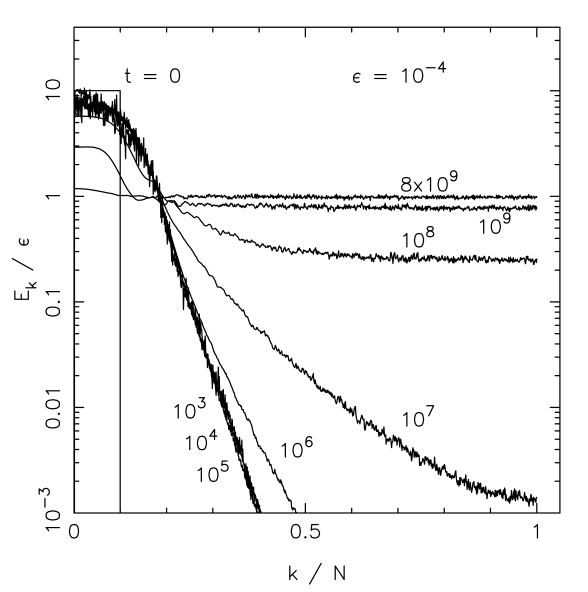
\includegraphics[width=0.4\textwidth]{./figs/FPUT-1.png}%
	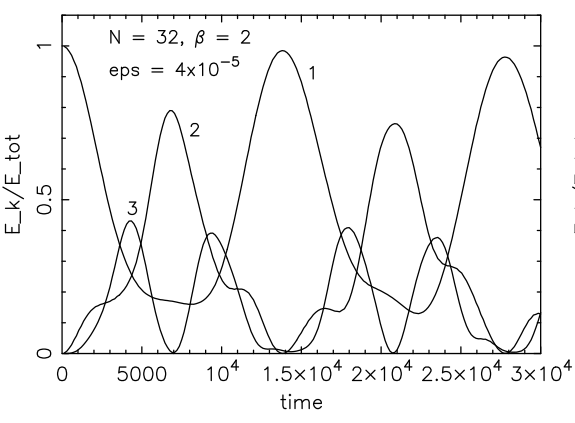
\includegraphics[width=0.5\textwidth]{./figs/FPUT-2.png}
	\caption{Averaged energy spectrum of normal modes $\bar{E}_k (T)$ plotted against $k/N$ at selected times $T$ and instantaneous values $E_k(t)$ for modes $k=1, 2, 3$ \cite{benettinFermiPastaUlamProblemIts2013}.}
	\label{fig:}
\end{figure}

System shows periodicity instead of equipartition of energy! Why? Are there some hidden symmetries? Still today, there is no satisfactory explanation for FPUT paradox. The FPUT system is close to a class of so-called \textit{integrable models}, whose a number of (hidden) symmetries, roughly speaking, is the same as the degrees of freedom. 

One obtains FPUT model by introducing perturbation to harmonic oscillator (which is integrable). By truncating FPUT model, one has Toda chain. Taking the continuum limit, FPUT model leads to Korteweg-de Vries (KdV) equation, which is integrable. This lecture is about these integrable models with ``large'' number of symmetries, about mathematical formulation and implications.

About literacy ``integrable'': There is possibility to integrate equation of motion to obtain a solution in a form as closed as possible (may require some extra steps).

\chapter{Integrability in classical mechanics}
\section{Hamiltonian Formalism}
Motion of a system with $n$ degrees of freedom described by trajectory in $2$ dimensional phase space $\mathcal{M}$ (manifold) with \textbf{local} coordinates $(p_j, q_j), j=1,\dots, n$.

\paragraph{Dynamical variables} are some function $f: \mathcal{M}\times \R \rightarrow \R, f=f(p, q, t)$.

\paragraph{Poisson brackets}
\begin{equation}
	\left\{f, g  \right\} := \sum_{i=1}^{k} \pdv{f}{q_k} \pdv{g}{p_k} - \pdv{f}{p_k}\pdv{g}{q_k}
\end{equation}
with the properties
\begin{align*}
	\pb{f}{g} &= - \pb{f}{g}  \\
	\pb{f}{\pb{g}{h}} &+ \pb{g}{\pb{h}{f}} + \pb{h}{\pb{f}{g}}  = 0
	\label{eq:}
\end{align*}
and the canonical ``commutation'' relation
\begin{equation*}
	\pb{p_j}{p_k} 	 = \pb{q_j}{q_k}  = 0, \quad \pb{p_j}{q_k}  = \delta_{jk}
\end{equation*}

Given a Hamiltonian $H = H(p, q, t)$, the dynamics of a dynamical variable is determined by 
\begin{equation*}
	\dv{f}{t} = \pdv{f}{t} + \pb{f}{H}	
\end{equation*}
for any $f = f(p, q)$.

Setting $f=p_j$ or $f=q_j$ yields the Hamilton's equation of motion
\begin{equation}
	\dot{p}_j = - \pdv{H}{q_j}, \quad \dot{q}_j = \pdv{H}{p_j}
	\label{math:ham-eom}
\end{equation}
The system \eqref{math:ham-eom} of $2n$ ordinary differential equations (ODEs) is deterministic, meaning the $(p_j(t), q_j(t))$ are uniquely determined by $2n$ initial conditions.

\begin{definition}
	A function $f= f(p_j, q_j, t)$ which $\dot{f} = 0$, when equation of motion \eqref{math:ham-eom} hold, is called	a \textbf{first integral}, a \textbf{constant of motion}, or a \textbf{conserved charge}.
\end{definition}
Equivalently, $f(p(t), q(t), t) = \text{const}$, if $p(t)$ and $q(t)$ satisfy \eqref{math:ham-eom}.

Hamilton's equations will be solvable, if there are ``sufficiently'' many constants of motion.

\paragraph{Example}
	System with one degree of freedom with $\M = \R^2$ and Hamiltonian $H = \frac{1}{2} p^2 + V(q)$. The Hamilton's equations are
	\begin{equation*}
		\dot{q} = p, \quad \dot{p} = - \pdv{V}{q}	.
	\end{equation*}
	The Hamiltonian $H$ is a first integral	 ($\dv{H} = 0$). Thus,
	\begin{align*}
		\frac{1}{2} p^2 &+ V(q) = E = \text{const} , \\
		\dot{q} &= p, p = \pm \sqrt{2(E-V(q))} , \\
		\Rightarrow t &= \pm \int \frac{\dd{q}}{\sqrt{2(E-V(q))}}
	\end{align*}
	Explicit solution could be found if the integral can be performed and the relation $t=t(q)$ can be inverted to get $q(t)$. These two steps are not always possible, but still it is called \textbf{integrable}.

One can also look at the systems \textbf{geometrically}. First integrals defines $f(p, q)=\text{const.}$ in $\M$. Two hypersurfaces corresponding to two first integrals generically intersect in surface of dimension $2$ in $\M$. In general, trajectory lies on a surface of dimension $(2n-L)$ with $L$ the number of independent first integrals. If $L=2n-1$, this ``surface'' is a curve, i.e. a solution to Hamilton's equations.

The questions now is how to find first integrals? If two first integrals are given, their Poisson bracket is another first integral. Noether's theorem gives first integrals (translations, rotations and so on). Energy is always a first integral in Hamilton formalism.

\section{Integrability and action-angle variables}
\begin{definition}
	Consider a Hamiltonian system with $2n$ dimensional phase space $\M$. We call this system (completely) Louville integrable, if $n$ functions $f_1, \dots, f_n: \M \rightarrow \R$ exists such that
	\begin{itemize}
		\item $\pb{f_j}{f_k} = 0, j, k = 1, \dots, n$
		\item $\pb{H}{f_j} = 0, j=1, \dots, n$
		\item The functions $f_1, \dots, f_n$ are independent, i.e. the $\vec{\nabla} f_j$ are linearly independent vectors on a tangent space to any point in $\M$.
	\end{itemize}
\end{definition}
If condition $(1)$ is satisfied, the $f_j$ are in \textbf{involution}. Integrability in the above sense leads to solvability of equation of motion.

\paragraph{Coordinate transformations}
What freedom is there in Hamiltonian structure?

\begin{definition}
	A transformation $Q_k = Q_k(p, q), P_k = P_k(p, q)$ is canonical, if it preserves the Poisson brackets
	\begin{equation*}
		\pb{f}{g}_{p, q} = \pb{f}{g}_{P, Q}, \forall f,g: \M \rightarrow \R.
	\end{equation*}
\end{definition}
Canonical transformation preserves Hamilton's equations. In $2n$ dimensional phase space, only $2n$ of the coordinates $p, q, P, Q$ are independent. Given a generating function $S(q, P, t)$ with
\begin{equation*}
	\det(\pdv[2]{S}{q_i}{p_k}) = 0	
\end{equation*}
we can construct a canonical transformation by setting 
\begin{equation}
	p_k = \pdv{S}{q_k}, \quad Q_k = \pdv{S}{P_k}, \quad H = H+ \pdv{S}{t}
\end{equation}
There are other possibilities with
\begin{align*}
	S(q, Q):& \; p = \pdv{S}{q} , P=-\pdv{S}{Q} , \\
	S(p, Q):& \; P = -\pdv{S}{Q}, q = - \pdv{S}{Q}, \\
	S(p, P):& \; q = - \pdv{S}{p}, Q= \pdv{S}{P}
	\label{eq:}
\end{align*}
Can we find canonical transformation that manifests integrability such that $P_k(t) = P_k(0) =\text{const}$ $n$ constant of motion and $Q_k(t) = Q_k(0) + t \pdv{H}{p_k}$ with linear time dependence. To find such a transformation is in general hard. Deciding whether a given $H$ is integrable is still unsolved problem.

\begin{theorem} (Arnold and Liouville)
	Let $(\M, f_1, \dots, f_n)$ be an integrable system with a Hamiltonian $H=f_1$ and let	
	\begin{equation*}
		\M_f = \left\{ (p, q) \in \M \, |\, f_k (p, q) = c_k = \text{const},\, k=1, \dots, n \right\} 	
	\end{equation*}
	be a so-called $n$ dimensional level set of first integrals $f_n$.
	\begin{enumerate}
		\item if $M_f$ is compact and connected, then it is diffeomorphism to torus $T^n = S^1 \times \cdots \times S^1$.
		\item One introduces (in the neighborhood of this torus in $M$) the action angle variables 
			\begin{equation*}
				I_1, \dots, I_n, \quad \phi_1, \dots, \phi_n, \quad 0 \leq \phi_n \leq 2\pi	
			\end{equation*}
			such that the angles $\phi_k$ are coordinates on $M_f$ and the action (variable) $I_k=I_k(f_1, \dots, f_n)$ are first integrals.
		\item The canonical equations of motion \eqref{math:ham-eom} becomes
			\begin{equation}
				\dot{I}_k = 0, \quad \dot{\phi}_k = \omega_k (I_1, \dots, I_n), \quad k =1, \dots,n 
				\label{math:action-angle-eom}
			\end{equation}
			and the integrable system is solved by \textbf{quadratures} (finite number of algebraic equations and integrations of know functions).
	\end{enumerate}
\end{theorem}

\paragraph{Proof} (not to prove $(1)$ here). On $(2)$ and $(3)$

Motion takes place on surface of dimension $2n -n = n$
\begin{equation}
	f_1 (p,q) = c_1,\; \dots,\; f_n(p, q) = c_n .
	\label{math:arnold-theorem-first-integral}
\end{equation}
From $(1)$, this surface is a torus. Assume $\det(\pdv{f_i}{p_k}) \neq 0$ such that \eqref{math:arnold-theorem-first-integral} can be solved for the momenta $p_i = p_i (q, c)$ with $f_i(q, p(q,c )) = c_i$
\begin{align*}
	\pdv{q_j} & \Rightarrow \pdv{f_i}{q_j} + \sum_{k=0}^{n} \pdv{f_i}{p_k} \pdv{p_k}{q_j} = 0, \\
	 \sum_j \cdot \pdv{f_i}{p_j} &\Rightarrow \sum_j \pdv{f_m}{p_j} \pdv{f_i}{q_j} + \sum_{j, k} \pdv{f_m}{p_j}\pdv{f_i}{p_k} \pdv{p_k}{q_j} = 0, \\
	(mi) - (im) &\Rightarrow \pb{f_i}{f_m} + \sum_{j, k} \left( \pdv{f_m}{p_j} \pdv{f_i}{p_k} \pdv{p_k}{q_j} - \pdv{f_i}{p_j} \pdv{f_m}{p_k} \pdv{p_k}{q_j} \right)  = 0, \\
					&\Rightarrow \sum_{j, k} \pdv{f_i}{p_k} \pdv{f_m}{p_j} \left( \pdv{p_k}{q_j} - \pdv{p_j}{q_k} \right)  = 0, \\
	\left( \pdv{f_i}{p_k} \right) \text{ invertible} &\Rightarrow \pdv{p_k}{q_j} - \pdv{p_j}{q_k} = 0, \\
	\text{Stockes' theorem} &\Rightarrow \oint_{\mathcal{G}} \sum_{j=1}^{n} p_j \dd{q_j} = 0,
\end{align*}
for any closed curve on torus $T^n$ such are contractible to a point. On $T^n$ there are $n$ closed curves that cannot be contracted to a point, such that the corresponding integrals do not vanish.
\todo{Is compactness a condition for Stockes' theorem?}

\begin{definition}
\textbf{action variable}
\begin{equation}
	I_k := \frac{1}{2\pi} \oint_{\Gamma_k} \sum_{i=1}^{n} p_j \dd{q_j}, \quad k = 1, \dots, n
	\label{math:action-variable-def}
\end{equation}
where the curve $\Gamma_k$ is the $k$-th basic cycle on the torus $T^n$
\begin{equation*}
\Gamma_k = \left\{ (\tilde{\phi}_1, \dots \tilde{\phi}_n) \in T^n;\; 0 \leq \tilde{\phi}_k \leq 2\pi, \tilde{\phi}_j = \text{const, for} j\neq k  \right\}.
\end{equation*}

\end{definition}
$\tilde{\phi}_k$ denotes some coordinates on $T^n$. To find these coordinates is non-trivial, in practice it is not clear how to describe a torus explicitly. Arnold-Liouville theorem has character of existence theorem. \todo{why is it non-trivial? In 2d case, they can be parametrised easily.}

Stockes' theorem implies the action variables \eqref{math:action-variable-def} are independent of choice of $\Gamma_k$. The action variable \eqref{math:action-variable-def} are first integrals since $\oint p(q, c) \dd{q}$ only depend on $c_k = f_k$ and $f_k$'s are first integrals.

We have all the action variable in involution, since
\begin{align*}
	\pb{I_i}{I_j} &= \sum_{r, s, k} \left( \pdv{I_i}{f_r} \pdv{f_r}{q_k} \pdv{I_j}{f_s} \pdv{f_s}{p_k} - \pdv{I_i}{f_r} \pdv{f_r}{p_k} \pdv{I_j}{f_s} \pdv{f_s}{q_k} \right),  \\
					  &= \sum_{r,s} \pdv{I_j}{f_r} \pdv{I_j}{f_s} \pb{f_r}{f_s}, \\
					  &=0.
	\label{eq:}
\end{align*}
In particular $\pb{I_k}{H}=0$. 

The torus $\mathcal{M}_f$ can be equivalently defined ny 
\begin{equation*}
	I_1 = \tilde{c}_c, 	\dots, I_n = \tilde{c}_n
\end{equation*}
One may ask why is $I_k$ (as coordinate) better than $f_k$. If one defines $I_k = f_k$, the transformation $(p, q) \rightarrow (I, \phi)$ would not be canonical. 

Canonical angle coordinates $\phi_k$, which are the canonically conjugates to the actions via the generating functions
\begin{equation}
	S(q, I) = \int_{q_0}^{q} \sum_j p_j \dd{q_j},
\end{equation}
with $q_0$ some point on the torus. Modifying $q_0$ just adds a constant to $S$. The angle coordinates are
\begin{equation*}
	\phi_i = \pdv{S}{I_i}.
\end{equation*}
The angles are periodic. Consider two paths $C$ and $C \cup C_k$ (with $C_k = \Gamma_k$ the $k$-th cycle) between $q_0$ and $q$, see figure \ref{fig:torus-angle}.
\begin{figure}[ht]
	\centering
	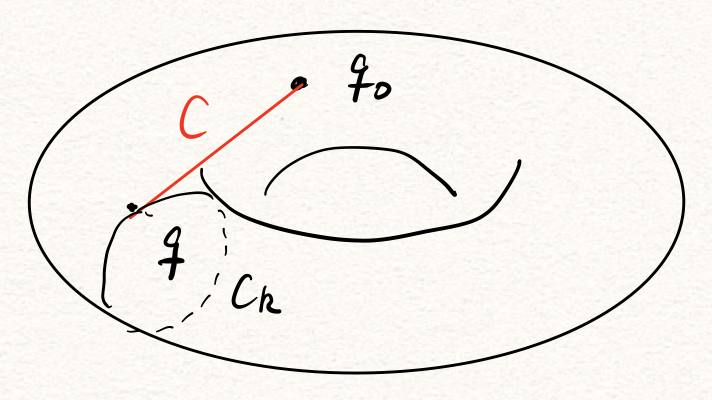
\includegraphics[width=0.4\textwidth]{./figs/torus-angle.jpg}
	\caption{Torus with two paths $C$ and $C\cup C_k$}
	\label{fig:torus-angle}
\end{figure}
Then
\begin{align*}
	S(q, I) &= \int_{C\cup C_k} \sum_j p_j \dd{q_j} \\
			  &= \int_{C} \sum_j p_j \dd{q_j} + \int_{C_k = \Gamma_k} \sum_j p_j \dd{q_j} \\
			  &= S(q, I) + 2\pi I_k \\
	\Rightarrow \phi_k &= \pdv{S}{I_k} = \phi_k + 2\pi
	\label{eq:}
\end{align*}

The transformation
\begin{equation*}
	q = q(\phi, I), \quad p = p(\phi, I)
\end{equation*}
and 
\begin{equation*}
	\phi = \phi(p, q) ,\quad I = I(p, q)
\end{equation*}
are canonical transformations (defined by the generating function $S$) and invertible. The Poisson structures are unchanged
\begin{align*}
	\pb{I_j}{I_k} = 0, \quad \pb{\phi_j}{\phi_k} = 0, \quad \pb{\phi_j}{I_k} = \delta_{jk}
	\label{eq:}
\end{align*}
The dynamics are given by
\begin{align*}
	\dot{\phi}_k = \pb{\phi_k}{\tilde{H}}, \quad \dot{I}_k = \pb{I_k}{\tilde{H}}
\end{align*}
with $\tilde{H} = \tilde{H}(\phi, I) = H(q(\phi, I), p(\phi, I))$. Since $I_k$'s are first integrals, 
\begin{equation*}
	0 = \dot{I}_k = \pdv{\tilde{H}}{\phi_k} ,
\end{equation*}
in other word $\tilde{H} = \tilde{H}(I)$. The derivatives of angle variable
\begin{equation*}
	\dot{\phi}_k = \pdv{\tilde{H}}{I_k} = \omega_k (I)
\end{equation*}
are first integrals as well.

Integration (``integrable'' model) yields
\begin{align}
	\begin{split}
		\phi_k (t) &= \omega_k(I) t + \phi_k (0), \\
		I_k(t) &= I_k(0).
	\end{split}
	\label{math:action-angle-sol}
\end{align}
The system is in a circular motion with constant angular velocity.

\paragraph{Geometric picture}
The phase space of an integrable system  is  foliated into an $n$-parameter ($c_j$) family of invariant tori on which flow is linear with constant frequency $\omega_k$. The trajectory \eqref{math:action-angle-sol} may be closed on the torus or it may cover it densely. For $n=2$, the trajectory is closed if $\omega_1/\omega_2$  is rational and dense otherwise.

\paragraph{Degeneracy}
The periodicity in $\phi$ means that every function $F(p, q)$ of the state of system is periodic in $\phi$. Expand the function in Fourier series, e.g. $n=2$
\begin{align*}
	F &= \sum_{l_1 = -\infty}^{\infty}\sum_{l_2 = -\infty}^{\infty} B_{l_1, l_2} \exp(i (l_1 \phi_1 + l_2\phi_2)), \\
	  &= \sum_{l_1, l_2} B_{l_1, l_2} \exp(it(l_1 \omega_1 + l_2 \omega_2)).
\end{align*}
Every summand is period with frequency $l_1\omega_1 + l_2\omega_2$. Sum of functions is not necessarily periodic. The whole sum is only periodic for rational $\omega_1 / \omega_2$. If $a_j \omega_j = a_k \omega_k$ for $a_{j, k} \in \Z$ for some $j, k$, one speaks of \textbf{degeneracy}. If $a_1\omega_1 = \dots = a_n \omega_n$, the system is \textbf{maximally} degenerate.

\paragraph{Example}
All time-indepedent Hamiltonian systems with $2$ dimensional phase-space are integrable ($H=f_{1=n}$). 

Consider a harmonic oscillator ($n=1$) with the Hamiltonian
\begin{equation*}
	H = \frac{1}{2} (p^2 + \omega^2 q^2)
\end{equation*}
Different choices of energy $c_1 = E$ give foliation of $\M$ by ellipses
\begin{equation*}
	\frac{1}{2} \left( p^2 + \omega^2 q^2 \right) 	 = E
\end{equation*}
with two axes $a = \sqrt{2E}$ and $b = \frac{\sqrt{2E}}{\omega}$ and surface $ab\pi$. For fixed $E$, take $\Gamma = \M_H$
\begin{equation*}
	I = \frac{1}{2\pi} \oint d\dd{q} \stackrel{\text{Stockes'}}{=} \frac{1}{2\pi} \int_{S} \dd{p} \dd{q} = \frac{E}{\omega}
\end{equation*}
The Hamiltonian in the new variable $\tilde{H} = \omega I$ and $\dot{\phi} = \pdv{\tilde{H}}{I} = \omega$, $\phi = \omega t + \phi_0$. 

To obtain the transformation $(p, q) \rightarrow (I, \phi)$, first the action variable is
\begin{equation*}
	I(p, q) = \frac{1}{\omega}H(p, q) = \frac{1}{2} \left( \frac{1}{\omega} p^2 + \omega q^2 \right) .
\end{equation*}
The generating function is
\begin{equation*}
	S(q, I ) = \int_{q_0}^{q} p \dd{\tilde{q}} = \pm \int_{q_0}^{q} \sqrt{2 I \omega - \omega^2 \tilde{q}} \dd{\tilde{q}}
\end{equation*}
and the angle variable
\begin{equation*}
	\phi = \pdv{S}{I} = \int \frac{\omega\ \dd{\tilde{q}}}{\sqrt{2I\omega - \omega^2 \tilde{q}^2}} = \arcsin(q \sqrt{\frac{\omega}{2I}}) - \phi_0.
\end{equation*}
Thus
\begin{align*}
	q &= \sqrt{\frac{2 E}{\omega}} \sin(\omega t + \phi_0) \\
	p &= \pdv{H}{p} = \dot{q} = \sqrt{2E} \cos(\omega t + \phi_0)
\end{align*}


%%%%%%%%%%%%%%%%%%%%%%%%%%%%%%%%%%%%%%%%%  lecture 3
\paragraph{Example} The Kepler Problem ($n=2$)

Consider the Motion in two-dimensional phase space (reduced from three-dimensional to two-dimensional using angular momentum conservation). Then we have four dimensional phase space $q_1 = \phi, q_2 = r, p_1 = p_\phi, p_2 = p_r$. The Hamiltonian is
\begin{equation*}
	H = \frac{p_\phi^2}{2r^2 } + \frac{p_r^2}{2} - \frac{\alpha}{r}
\end{equation*} 
with a positive constant $\alpha$. We have $\pb{H}{p_\phi} = 0$, the system is (Liouville) integrable ($2$ constants of motion). 

Level set $\M_f: H=E; p_\phi=\mu$. Then we can solve for $p_r$
\begin{align*}
	p_r = \pm \sqrt{2E - \frac{\mu^2}{r^2} + \frac{2\alpha}{r}}.
\end{align*}
$\phi$ is arbitrary, one constraint on $(r, p_r)$. Parametrize $\M_f$ by $\phi$ and function of $(r, p_r)$. Vary $\phi$ and fix other coordinate, consider one cycle $\Gamma_\phi \subset \M_f$
\begin{align*}
	I_\phi &= \frac{1}{2\pi} \oint_{\Gamma_\phi} \left( p_r \dd{r}+p_\phi \dd{\phi}  \right), \\
			 &= \frac{1}{2\pi} \int_0^{2\pi} p_\phi \dd{\phi} = \mu,
\end{align*}

To find the second action, fix $\phi$
\begin{align*}
	I_r &= \frac{1}{2\pi} \oint_{\Gamma_r} p_r \dd{r},	 \\
			 &= 2 \cdot \frac{1}{2\pi}\int_{r_-}^{r_+} \sqrt{2E - \frac{\mu^2}{r^2} + \frac{2\alpha}{r}} \dd{r},
\end{align*}
where we have taken the positive and negative roots and integrate $r_- \rightarrow r_+$ and backwards. Turning points $r_\pm$ are solutions of $2E - \frac{\mu^2}{r^2} + \frac{2\alpha}{r} = 0$ ($p_r \in \R$). Integral can be done using residual calculus 
\begin{equation*}
	I_r = \alpha \sqrt{\frac{1}{2 |E|}} - \mu = \alpha \sqrt{\frac{1}{2 |E|}} - I_\phi.
\end{equation*}
Thus, the Hamiltonian written in terms of actions is
\begin{align*}
	\tilde{H} &= - \frac{\alpha^2}{2(I_r + I_\phi)^2}, \\
	\Rightarrow \pdv{\tilde{H}}{I_r} &= \pdv{\tilde{H}}{I_\phi} = \frac{\alpha^2}{(I_r + I_\phi)^3}.
\end{align*}
This is a particular case with $\omega_r = \omega_\phi$, and therefore closed orbits.


\paragraph{Superintegrability} 
One may wonder why $\tilde{H} = \tilde{H}(I_r + I_\phi) $. Is there some special property in the system unexplored?  In general, an integrable system admits $n$ independent actions $I_k$, that can be uniquely expressed as functions of the system's state. We may write $(n-1)$ additional constants of motion as 
\begin{equation*}
	A_{ik} := \phi_i \pdv{H}{I_k} - \phi_k \pdv{H}{I_i}
\end{equation*}
remember $\dot{\phi_k} = \pdv{H}{I_k} = \omega_k$. Since $\phi_k = \phi_k + 2\pi$, the $A_{ik}$'s are not unique functions.

Suppose we have a degenerate system, e.g.
\begin{equation}
	a_1 \pdv{H}{I_2}	= a_2 \pdv{H}{I_2}
	\label{math:a_1_a_2}
\end{equation}
for $a_1, a_2 \in \Z$. Then 
\begin{equation*}
	B_{12} := a_1 \phi_1 - a_2 \phi_2,
\end{equation*}
is a constant of motion with $B_{12} = B_{12} + 2\pi n, n\in \Z$. Any trigonometric function of $B_{12}$ is unique constant of motion. Here \eqref{math:a_1_a_2} implies $H=H(a_2 I_1 + a_1 I_2)$. For the Kepler problem, the additional symmetry is the well-known \textbf{Laplace-Runge-Lenz vector}.

\begin{definition}
	A Hamiltonian system with $2n$-dimensional phase space and more than $n$ independent constants of motion is called \textbf{superintegrable}. If the system has $2n-1$ independent constants of motion, it is \textbf{maximally superintegrable}.
\end{definition}

\section{Poisson Structures}
Consider phase space $\M$ of dimension $m$ with local coordinates ($\xi^1, \dots, \xi^n$), where we make no distinction between coordinates and momenta.

\begin{definition}
	A skew-symmetric matrix $\omega^{ab} = \omega^{ab} (\xi)$	 is called a \textbf{Poisson structure}, if the Poisson bracket defined by 
	\begin{equation*}
		\pb{f}{g} =  \sum_{a, b = 1}^m \omega^{ab} (\xi) \pdv{f}{\xi^a} \pdv{g}{\xi^b}
	\end{equation*}
satisfies  $\pb{f}{g} = - \pb{g}{f}$ and the Jacobi identity.
\end{definition}
The Jacobi identity puts restrictions on $\omega^{ab}(\xi) = \pb{\xi^a}{\xi^b}$
\begin{align*}
	\sum_{d=1}^{m} \left( \omega^{dc} \pdv{\omega^{ab}}{\xi^d} + \omega^{db} \pdv{\omega^{ca}}{\xi^d} + \omega^{da} \pdv{\omega^{bc}}{\xi^d} \right) 	 = 0
\end{align*}

Given a Hamiltonian $H: \M \times \R \rightarrow \R$, the dynamics is given by
\begin{equation*}
	\dv{f}{t} = \pdv{f}{t} + \pb{f}{H}
\end{equation*}
and the Hamilton's equations generalizing \eqref{math:ham-eom} 
\begin{equation*}
	\dot{\xi}^a = \sum_{b=1}^m \omega^{ab}(\xi) \pdv{H}{\xi^b}
\end{equation*}

\paragraph{Example}
$\M = \R^3, \omega^{ab} = \sum_{c=1}^{3} \epsilon^{abc} \xi^c$, then
\begin{equation*}
	\pb{\xi^a}{\xi^b} = \epsilon^{abc} \xi^c = \sum \epsilon^{abc} \xi^c
\end{equation*}
This Poisson structure admits a Casimir, namaly any function $f(r)$, where
\begin{equation*}
	r = \sqrt{(\xi^1)^2 + (\xi^2)^2 + (\xi^3)^2},
\end{equation*}
and Poisson-commutes with the coordinate function $\pb{f(r)}{\xi^a}=0$.

\paragraph{Symplectic structures}
Assume $m=2n$ even and $\omega$ invertible with $W := \omega^{-1}$. Jacobi identity implies
\begin{equation*}
	\partial_a W_{bc} + \partial_c W_{ab} + \partial_b W_{ca} = 0,\quad \forall a, b, c = 1, \dots, m
\end{equation*}
In this case we call $W$ a \textbf{symplectic structure}.

The \textbf{Darboux theorem} states that there exists locally coordinate system with 
\begin{equation*}
	\xi^1 = q_1, \dots, \xi^n = q_n, \xi^{n+1} = p_1, \dots, \xi^{2n} = p_n
\end{equation*}
such that 
\begin{equation*}
	\omega = \begin{pmatrix} 0 & \id_n \\ -\id_n & 0 \end{pmatrix}
\end{equation*}
and the Poisson bracket reduces to the standard form.

\paragraph{Example} (Spinning Euler Top)

The coordinates are just the angular momentum $\xi^{1, 2, 3} = S^{x, y, z}$. The Hamiltonian is 
\begin{equation*}
	H = \frac{1}{2}\left[ \frac{(S^x)^2}{\Omega_x} + \frac{(S^y)^2}{\Omega_y} + \frac{(S^z)^2}{\Omega_z}\right] 
\end{equation*}
for angular momentum vector $\vec{S}$ of a rigid spinning body fixed at center of mass. $\Omega_i$ is the diagonal entry of moment of inertia matrix $\Omega$, such that $\vec{S} = \Omega \vec{\omega}$ with $\vec{\omega}$ the angular velocities. 

Hamilton's equations (Euler equations) are
\begin{equation*}
	\dv{t} \vec{S} = - \pb{H} {\vec{S}} = \left( \Omega^{-1} \vec{S} \right)  \times \vec{S}.
\end{equation*}
(Sometimes written as three decoupled differential equations.)

There are two conserved charges $H$ and $|\vec{S}|$. Use $H = E$ and $|\vec{S}|=l$ to write the equation of motion as 
\begin{equation*}
	\dv{t} S_x = \sqrt{A + B S_x^2 + C S_x^4}
\end{equation*}
with $A, B, C$ functions of $\Omega, l , E$. Extinguish three cases
\begin{table}[ht]
	\centering
	\label{tab:label}
	\begin{tabular}{c c c c}
	\toprule
	solution & rational & trigonometric & elliptic \\
	\midrule
	name & $x x x$ & $x x z$ & $x y z$ \\
	$\Omega_{x, y, z}$ & $\Omega_x, \Omega_x, \Omega_x$ & $\Omega_{x}, \Omega_x, \Omega_z$ & $\Omega_x, \Omega_y, \Omega_z$ \\
	symmetry & $\SO(3)$ & $\SO(2)$ & $-$ \\
	\bottomrule
	\end{tabular}
	\caption{}
\end{table}

\section{Classical chains and Fields}
We can align elementary mechanical models on a one dimensional lattice and it yields a chain model. Examples are FPUT, Toda chain, classical spin chain. Infinite chains have infinitely many degrees of freedom. The question is how many (conserved) charges do we need for integrability? Precise meaning of integrability is not clear, won't discuss classical field here.

\paragraph{Continuum limits} 
Field theories are naturally understood as continuum limits of lattice models (chain). A well-behaved continuum limit of an integrable lattice model should be integrable.

General idea is to consider one dimensional classical chain model of variable $\xi_j$. Sites are labelled by $j$ at position $x_j = x + j\cdot a$ with a constant lattice spacing $a = x_{j+1}  - x_j$. Continuum limit $a\rightarrow 0$. Fix limiting continuous field $\phi(x)$ via 
\begin{equation*}
	\xi_j = X_j (a, \phi(x_j))
\end{equation*}
with $X_j$ some function specifies the limit prescription (There is no well-defined continuous limit!).

The Simplest example is $\xi_j = \phi(x_j)$. In the limit $a\rightarrow 0$ for instance 
\begin{align*}
	\phi'(x) &= \lim_{a\rightarrow 0} \frac{\phi(x_{j+1}) - \phi(x_j)}{a}, \\
	\phi''(x) &= \lim_{a\rightarrow 0} \frac{\phi(x_{j+1}) - 2 \phi(x_j) + \phi(x_{j-1})}{a^2}, \dots
\end{align*}
Lattice sums turn into integrals
\begin{equation*}
	\lim_{a\rightarrow 0} a \sum_j (\dots) = \int \dd{x} \dots .
\end{equation*}
Delta function becomes kronecker delta
\begin{equation*}
	\delta(x-y) = \lim_{a\rightarrow 0} \frac{1}{a} \delta_{jk}
\end{equation*}
May have expressions including different points $x_j = x+ja$ and $x_k = y+ka$, such that 
\begin{equation*}
	x = \lim_{a\rightarrow 0} (x_0 + ja), y = \lim_{a\rightarrow 0} (x_0 + ka)
\end{equation*}
Definition of integrability for field theory is even worse than chain models.


%%%%%%%%%%%%%%%%%%%%%%%%%%%%%%%%%%%%%%%%%%%%%%% lecture 4

\paragraph{Hamiltonian formalism for fields}
Formally, replace coordinates $\xi (t)$ by field variable $\phi(t, x)$, replace phase space $\M(=\R^m)$ by space of smooth functions on a line $(=\R)$ with some boundary conditions (e.g. decay, open, periodic). 
\begin{table}[htpb]
	\centering
	\begin{tabular}{cc}
		\toprule
		elementary mechanics & fields \\
		\midrule
		$\xi^a(t), a = 1, \dots, m$ & $\phi(t, x), x\in \R$ \\
		$\sum_a$ & $\int_{\R}\dd{x}$ \\
		function $f(\xi)$ & functional $F[\phi]$ \\
		$\pdv{\xi^a}$ & $\fdv{\phi}$ \\
		ODEs $(t)$ & PDEs $(t, x)$ \\
		\bottomrule
	\end{tabular}
	\caption{}
\end{table}

Functionals given by integrals
\begin{equation*}
	F[\phi] = \int_{\R} f(\phi, \phi_x, \phi_{x x }, \dots) \dd{x}
\end{equation*}
Recall 
\begin{equation*}
	\fdv{F}{\phi(x)} = \pdv{f}{\phi} - \pdv{x} \pdv{f}{\phi_x} + \pdv[2]{x} \pdv{f}{\phi_{x x}}
\end{equation*}
and 
\begin{equation*}
	\fdv{\phi(y)}{\phi(x)} = \delta(x-y)
\end{equation*}
with $\int_{\R} \delta(x) \dd{x} = 1$.

\begin{definition}Poisson bracket in this case can be defined as 
	\begin{equation*}
		\pb{F}{G} = \int_{\R} \omega(x, y, \phi) \fdv{F}{\phi(x)} \fdv{G}{\phi(y)} \dd{x} \dd{y}
	\end{equation*}
with $\omega$ such that the Poisson bracket is anti-symmetric and obeys Jacobi-identity.
\end{definition}

Canonical choice
\begin{equation*}
	\delta(x, y, \phi) = \frac{1}{2} \partial_x \delta(x-y) - \frac{1}{2} \partial_y \delta(x-y)
\end{equation*}
It is analogous to Darboux form, where $\omega$ is constant and anti-symmetric. Antisymmetry is analogous to $\pdv{x}$ being anti-self-dual with respect to inner product $\langle \phi, \psi \rangle = \int_{\R} \phi(x) \psi(x) \dd{x}$. 

Hence, the canonical bracket is 
\begin{equation*}
	\pb{F}{G} = \int_{\R} \fdv{F}{\phi(x)} \pdv{x} \fdv{G}{\phi(x)} \dd{x}
\end{equation*}
with Hamilton's equations 
\begin{equation}
	\pdv{\phi}{t} = \pb{\phi}{H[\phi]}.
\end{equation}

\printbibliography
\end{document}
